\documentclass[12pt]{report}

%---------------------------------------------------------------
% Package Inclusions
\usepackage[svgnames]{xcolor}
\usepackage{booktabs}
\usepackage{fancyhdr}
\usepackage{paralist}
\usepackage{graphicx}		
\usepackage{amsmath}		
\usepackage{amssymb}	
\usepackage{amsthm}
\usepackage{tikz}
\usetikzlibrary{shadows,positioning,arrows,fit,petri,decorations.pathmorphing,backgrounds}

%---------------------------------------------------------------
% Page Layout
\pagestyle{fancy}
\setlength{\parindent}{0 pt}
\oddsidemargin = .5 in
\textheight = 560pt
\textwidth = 5.5 in
\headwidth = \textwidth

%---------------------------------------------------------------
% Verbatim Text
\usepackage{fancyvrb,fancybox,calc} 
\usepackage[svgnames]{xcolor} 
\newenvironment{code}{\VerbatimEnvironment%
  \begin{Sbox} 
  \begin{minipage}{\linewidth-2\fboxsep-2\fboxrule-4pt}    
  \begin{Verbatim}
}{% 
  \end{Verbatim}
  \end{minipage}   
  \end{Sbox}
  \fcolorbox{black}{LightGray}{\TheSbox} 
} 

%------------------------------------------------------------------
% Header Format
\lhead{}
\renewcommand{\headrulewidth}{.4pt}
\renewcommand{\footrulewidth}{.4pt}

%------------------------------------------------------------------
% OTHER FORMATTING
\setcounter{tocdepth}{1}
\setlength{\parskip}{5pt}
\newenvironment{grammar}{\begin{center}\itshape \begin{tabular}{l}}{\end{tabular}\end{center}}
\newenvironment{myList}
{\begin{itemize}
  \setlength{\itemsep}{3pt}
  \setlength{\parskip}{0pt}
  \setlength{\parsep}{0pt}}
{\end{itemize}}

\newenvironment{myNumList}
{\begin{enumerate}
  \setlength{\itemsep}{3pt}
  \setlength{\parskip}{0pt}
  \setlength{\parsep}{0pt}}
{\end{enumerate}}

%------------------------------------------------------------------
% CUSTOM COMMANDS
\newcommand{\set}[1]{\lbrace #1 \rbrace}
\newcommand{\OR}{$\phantom{x}\vert\phantom{x}$}

%------------------------------------------------------------------
% Global Vars
\def \lang {{\scshape Setup} }

\title{\scshape \Huge The Setup Programming Language
\author{Ian Erb (ire2102)\\
Bill Warner (whw2108)\\
Adam Weis (ajw2137)\\
Andrew Ingraham (aci2110)
}
\date{\today}
}

%---------------------------------------------------------------------------
% DOCUMENT BEGINS

\begin{document}
\maketitle
\tableofcontents

%----------------------------------------------------------------------------
% Language Reference Manual
\chapter{Introduction}
The \lang language was created to leverage the clear and concise syntax of set formalisms in mathematics.  With \lang, users can generate sets using a variety of logic and combinatorial techniques that would require significantly more lines of code in other imperative languages such as Java, C or C++.  \lang was designed with the following goals in mind:
\begin{itemize}
\item\textbf{Set Theory Abstraction. }\lang provides a framework for handling data which many mathematicians and scientists will find familiar and easy to use.  By maintaining a sufficient level of abstraction, \lang can minimize the time needed to go from concept to concrete, working code.  

\item \textbf{Minimal Code Generation. } \lang greatly reduces the amount of code needed to perform routine tasks.  The user will find that nested loops can be virtually eliminated from code, making program files lighter and debugging easier.

\item \textbf{High Level of Readability. } \lang aims to be a clear and concise programming language with intuitive commands and syntax which mirror the mathematical underpinnings of set theory.
\end{itemize}
\chapter{Setup Tutorial}
Each program you write in \lang should be placed in a plain text file.  By convention, the \verb|.su| suffix is used to denote programs written in valid \lang code.  Let's write a simple program to get the hang for how \lang works.

\section{A Simple Scheduling Program}
\subsection{Writing the Code}
Create a text file entitled \verb|schedule.su| and open it in your text editor.  In this file, place the following text:

\begin{code}
/* Our First Program */
function main[] returns int {
   set days = {"M","T","W","Th","F"};
   set hrs = {1...24};
   set week = Days cross hrs;
   return 0;   
   }
\end{code}

We use the keyword \verb|set| to indicate that we are defining a variable name for a set
\subsection{Compiling a Program}

\begin{code}

-$ ./cWriter.native < hello.su

\end{code}

\section{Sets and Tuples}
\section{Using Set-Builder Notation}

\chapter{Language Reference Manual}
\section{Overview}
\subsection{Introduction}
The language of set theory is widely used by mathematicians and scientists to construct and manipulate large collections of objects in an abstract setting.  The \lang language implements the most useful and commonly used abstractions (e.g., union, intersections, direct products) from set theory in a language which users of other common imperative languages such as C, C++ and Java will find very simple and intuitive.

\lang was created with three goals in mind:
\begin{myNumList}
	\item Construct sets in a logical way
	\item Perform operations on large sets with minimal code generation 
	\item Maintain a high level of readability
\end{myNumList}

We anticipate users will solve simple set-oriented problems like scheduling, logic, and probability problems.

\subsection{A Motivating Example}
\lang greatly reduces the amount of code required to generate and manipulate sets.  A level of abstraction is provided which allows the user to work with sets in an intuitive way -- simultaneously improving readability. For example, the need for writing successive nested loops is practically eliminated.

Suppose the user wanted to generate all possible ordered pairs of numbers from 1 to 10.  In C++, we would write:

\begin{code}
struct { int first; int second; } pair;
vector<pair> pairs;
for(int i = 1; i!= 11; i++){
    for(int j = 1; j!=11; j++){
		pair temp;
		temp.first = i;
		temp.second = j;        
        vector.push_back(temp); 
    }
}
\end{code}

In \lang , the equivalent code can be written:

\begin{code}
set A = {1...10};
set pairs = {(x,y) | x in A, y in A};
\end{code}

Making use of \verb|cross| -- a built-in cartesian product operator -- we can further simplify our code to a single line:

\begin{code}
set pairs = {1...10} cross {1...10};
\end{code}

Though somewhat trivial, the above example shows how we can greatly reduce code and improve readability at the same time.  Suppose we wanted to remove duplicates \verb| (1,1) ... (10,10)|.  We would simply write

\begin{code}
set unique_pairs = pairs minus {(x,x) | x in {1...10}};
\end{code}

Here we highlight another useful built in operator -- \verb| minus | -- which returns the complement of the second set within the first set.  That is, \verb| A minus B| $= A \cap B^c.$  

Working with \lang is simple and getting started is easy.

\subsection{Lexical Conventions}
The language has 5 basic tokens: 
\begin{myList}
	\item Identifiers
	\item Keywords
	\item Literals
	\item Operators
	\item Punctuation
\end{myList}
Whitespace characters (blanks, tabs and newlines) are ignored and used only to separate tokens.  At least one whitespace character is required to separate adjacent tokens.

\subsubsection{Comments}
Block comments are introduced with \verb|/*| and terminated with \verb|*/|.  Nesting of comments is not permitted.  Comments are in general ignored by the compiler.

\subsubsection{Identifiers}
\label{id}
An identifier is a sequence of letters and digits.  The first character must be alphabetic.  Names are case-sensitive.
	
\subsubsection{Keywords}
The following identifiers are reserved for use as keywords, and may not be used otherwise:
	\begin{center}
	\begin{tabular}{lllll}
	\verb|set|\qquad\qquad\qquad &\verb|int| \qquad\qquad\qquad &\verb|bool| \qquad\qquad\qquad &	\verb|float| \qquad\qquad\qquad &\verb|string| \\
	\verb|if| &\verb|tuple| &\verb|in| &\verb|then| &\verb|union|\\
	\verb|else| &\verb|intersect| &\verb|minus| &\verb|while| &\verb|cross|\\
	\verb|true| &\verb|function| &\verb|returns| &\verb|false| &\verb|return|
	\end{tabular}
	\end{center}

\subsubsection{Primitive Types}
	There are four primitive types in \lang:  	
		\subsubsection{Integers}
		An integer is a sequence of digits.  All integers are lexed as a sequence of digits with an optional leading minus sign for negative integers.  They are represented internally using architecture native integer representation.
		\subsubsection{Strings}
		A string is a sequence of characters enclosed in double quotes as in \verb|"string"|.  Two adjacent strings are concatenated using the "+" sign.  As in
		\begin{center}
		\verb|"string" + "concat" -> "stringconcat"|.
		\end{center}
		\subsubsection{Floats}
		We adopt the \textit{C Reference Manual} definition of a floating point number:
		\begin{quotation}
		A floating constant consists of an integer part, a decimal point, a fraction part, an \verb|e| and an optionally signed integer exponent.  The integer and fraction parts both consist of a sequence of digits.  Either the integer part or the fraction part (not both) may be missing; either the decimal point or the \verb|e| and the exponent (not both) may be missing.
		\end{quotation}		
		All floating point numbers will be 64-bit double precision.
		\subsubsection{Booleans}
		A Boolean value can take either \verb|true| or \verb|false|.

\section{Syntax Notation}
In this manual, elements of language syntax are indicated by \textit{italic} type.  Literal words and characters are written in \verb|verbatim|.  Alternatives are listed using the "$\lvert$" character: $\textit{item $\lvert$ item}$.

\section{Objects}
\subsection{Variables}
A variable token is an identifier to a stored primitive, tuple or set.  A variable must begin with an alphabetic character followed by zero or more letters and digits.  Variables are declared by referencing their type followed by the associated token and an optional initializer, as in \verb|int a;| or \verb|int a = 3;|.  All global variables must be declared outside of any function definition, and cannot include an initializer.
	
A variable, once declared, may be reassigned but cannot be declared again in the same scope.
	
\begin{code}
int a = 3;
a=4;         /* ok    */
int a = 5;   /* error */
\end{code}
	
	\subsubsection{Variable Initialization}
	Variables for primitives not explicitly initialized when declared will be initialized as follows:
	\begin{align*}
	&int \to 0\\
	&string \to ""\\
	&float \to 0.0\\
	&bool \to false\\
	&set \to \set{}
    \end{align*}
	Uninitialized tuples are not permitted.

\subsection{Tuples}
A \textit{n-tuple} is an ordered collection of $n$ comma-delimited \textit{expressions} enclosed in parentheses.  An 		\textit{element} is either a primitive, set or tuple.  An \textit{n-tuple} and \textit{m-tuple} are considered of the 			same type if the following two conditions are satisfied:
		\begin{itemize}
		\item $n = m$.
		\item The type of each coordinate \textit{element} is of the same type.
		\end{itemize}
	For example, the following tuple elements are not the same type because the first coordinate \textit{tuples} are not of the same \textit{type}:
	
\begin{code}
((1,"a"),2) //type: ((int,str),int)
((1,2),3) //type: ((int,int),int)
\end{code}
	
\subsection{Sets}
A set is an unordered collection (potentially empty) of terminals, sets or tuples.  Every element of a set is unique (duplicate elements are discarded).  A set must be \textbf{homogeneous in type}, meaning that every element within the set has matching type.  All sets are typed as \verb|set|, regardless of their contents.  This means that a set containing sets of varying types is allowed.  

\begin{code}
{1,2,3,4} /* valid: homogeneous in type */
{1,2,3,"f"} /* invalid: not homogeneous in type */
{(1,2),(3.0,4.0)} /* invalid: tuple types are deep */
{{1,2,3},{"a","b"}} /* valid: set types are shallow */
\end{code}

Sets can be initialized in various ways:
	\subsubsection{Literal Initialization}
	A set may be initialized with a comma-delimited list of elements or identifiers of matching type within curly braces:
	
\begin{code}	
set A = {1, 2, 3, 4, 5, 6}; /* ok */
string b = "name";
set B = {"this", "works", b}; /* ok */
set C = {1, 2, 3, b}; /* error: type mismatch */
\end{code}

	\subsubsection{Range Initialization}
	For sets of integer type, we allow the following range initialization using "\verb|...|":

\begin{code}	
set A = {1 ... 6}; /* ok: returns {1, 2, 3, 4, 5, 6} */
set B = {1 ... 3, 5...7}; /* ok: returns {1, 2, 3, 5, 6, 7} */
set C = {3 ... -1}; /* ok: returns {3, 2, 1, 0, -1} */
\end{code}
		
	\subsubsection{Set-Builder Initialization}
	The following syntax is used for initializing a set through set-builder notation:
	\begin{grammar}
	\verb|{| expr pipe sourcelist \verb|}|
	\end{grammar}
	The source list is a sequence of comma-delimited expressions of the form 
	\begin{center}
	$id$ \verb|in| $set$  
	\end{center}	
	Each $id$ represents a local variable which may be used to construct new elements for a set via the expression appearing on the left hand side of the $\vert$ symbol.  The sequenced sourcelist expressions are evaluated left-to-right.  
	
	The \verb|in| operator is right associative, and the $id$ is not assigned a value until the right operand has been resolved.  The resulting set will include the resulting left side expression evaluated for all potential $id$ values, with duplicates removed.

\begin{code}
set A = { (x,y) | x in {1,2,3}, y in {"a","b","c"} };
B = { (1,"a"),(1,"b"),(1,"c"),
      (2,"a"),(2,"b"),(2,"c"),
      (3,"a"),(3,"b"),(3,"c") };
A == B; /* returns yup */
\end{code}

In addition, the left side expression may contain references to variables in enclosing scopes (local sourcelist variables shadow enclosing scopes).  For example:

\begin{code}
int a = 0;
int x = 5;	
set A = { (a,x) | x in {1,2,3} }; /*x shadows enclosing x = 5*/
B = { (0,1),(0,2),(0,3) };
A == B; /*returns yup*/
\end{code}

\section{Operators}
\subsection{Arithmetic Operations}
The following arithmetic operations are provided: \verb|+,-,*| for types \verb|int| and \verb|float|. The return type is as follows:
	\begin{align*}
		&\textit{int binop int $\to$ int}\\
		&\textit{float binop float $\to$ float}\\
		&\textit{float binop int $\to$ float}\\
		&\textit{int  binop float $\to$ float}
	\end{align*}
There are two division operators:
\begin{enumerate}
\item
\verb|/|, which accepts as arguments any two numerical values and is guaranteed to return a \verb|float| 
\item 
\verb|//| accepts as arguments any two numerical values and is guaranteed to return an \verb|int| truncated toward zero. 
\end{enumerate}
  
	
The following relational operators are provided for all primitive types: \verb|<,>,<=,>=,==,!=|.  Types passed to these operators must match, except in the case of \verb|<,>| when comparing \verb|int| and \verb|float|.  String comparison is done lexicographically as per \verb|strcmp| in the $C$ standard library.  The only character set supported is 8-bit ASCII.

\subsection{Set Operations}
The following set operations are provided:
	\begin{center}	
	\begin{tabular}{lllll}
	\verb|union| &\verb|intersect| &\verb|minus| &\verb|cross| &\verb|#|
	\end{tabular}
	\end{center}
\subsubsection*{union}
\verb|union| is a binary operator which returns a union of two sets.  Both sets must contain elements of the same type.
\subsubsection*{intersect}
\verb|intersect| is a binary operator which returns the intersection of two sets.  Both sets must contain elements of the same type.
\subsubsection*{minus}
\verb|minus| is a binary operator which returns a set of elements which are present in the first set but \textbf{not} in the second set.  Both sets must contain elements of the same type.

\subsubsection*{cross}
\verb|cross| takes as left operand a set with elements of type $a$ and as right operand a set of elements with type $b$ and returns an exhaustive set of tuples of type $(a,b)$, duplicates removed.

\subsubsection*{\#}
\verb|#| is a unary operator returning the number of elements in a set.  

\section{Language Syntax}
\subsection{Structure of a Setup Program}
Every \lang progam is a sequence of zero or more function definitions and/or variable declarations.  Variable declarations outside of function bodies are considered global in scope and may not be assigned a value when declared.
\begin{grammar}
program $\to \epsilon$\\
program $\to$ funcdef program\\
program $\to$ vdecl program
\end{grammar}
Execution (of non-empty programs) begins by calling the \verb|main| function which returns an \verb|int|.  User-defined functions must be defined before the \verb|main| function.  Nested function definitions are not permitted.

\subsection{Expressions}
\subsubsection*{Terminals}
\begin{grammar}
expr $\to$ float \OR int \OR string \OR bool \OR id
\end{grammar}
\subsubsection*{Tuples}
\begin{grammar}
expr $\to$ tuple\\
tuple $\to$ \verb|(| expr-list \verb|)|\\
expr-list $\to$ expr \OR expr\verb|,|expr-list 
\end{grammar}
\subsubsection*{Sets}
\begin{grammar}
expr $\to$ set\\
set $\to$ \verb|{| expr-list \verb|}|\\
set $\to$ \verb|{| int \verb|...| int \verb|}|\\
set $\to$ \verb|{| expr $\vert$ source-list \verb|}|\\
source-list $\to$ id \verb|in| expr \OR id \verb|in| expr, source-list
\end{grammar}

\subsubsection*{Operations}
\begin{grammar}
expr $\to$ id \verb| = | expr\\
expr $\to$ expr binop expr\\
expr $\to$ unop expr\\
\end{grammar}

\subsection{Functions}
Function definitions begin with the keyword \verb|function| followed by a valid identifier (see \ref{id}), a possibly empty list of formals, a return type specified using the keyword \verb|return| and a curly-brace enclosed list of statements.
\begin{grammar}
funcdef $\to$ \verb|function| id \verb|[| formals-list \verb|] returns| typespec \verb|{| stmt-list\verb| }|\\
formals-list $\to \epsilon$ \OR formals-tail\\
formals-tail $\to$ formal \OR formal formals-tail\\
\textit{formal $\to$ typespec id}\\
\textit{typespec $\to$} \verb|int| $\vert$ \verb|set| $\vert$ \verb|float| $\vert$ \verb|string| $\vert$ \verb|tuple| $\vert$ \verb|bool|
\end{grammar}
Function definitions specify the expression to be returned using a return statement:
\begin{grammar}
\verb|return | expr\verb|;|
\end{grammar}
Functions are called by specifying an $id$ and a list of arguments enclosed in parentheses:
\begin{grammar}
funcall $\to$ id\verb|( |arglist\verb| )|\\
arglist $\to \epsilon$ \OR exprlist\\
exprlist $\to$ expr \OR expr \verb|,| exprlist
\end{grammar}

\subsection{Statements}
A statement list is simply a sequence of one or more statements:
\begin{grammar}
stmt-list $\to$ stmt \OR stmt stmt-list
\end{grammar}
with the following valid statements:
\subsubsection*{Variable Declaration and Assignment}
\begin{grammar}
stmt $\to$ typespec id\verb|;|\\
stmt $\to$ typespec id\verb| =| expr\verb|;|\\
\end{grammar}
\subsubsection*{Control Statements}
\begin{grammar}
stmt $\to$ \verb|if(| expr \verb|) then| \verb|{| stmt-list\verb| } else {| stmt-list\verb| }|\\ 
stmt $\to$ \verb|while (| expr \verb|) {| stmt-list \verb|}|\\
stmt $\to$ \verb|return (| expr \verb|);|\\
\end{grammar}Definitions
\subsubsection*{Print Statement}
\lang provides a method for nice printing to the standard output:
\begin{grammar}
stmt $\to$ \verb|Print (| expr \verb|);| 
\end{grammar}
\subsubsection*{Expressions}
A statement may also be an expression:
\begin{grammar}
stmt $\to$ expr\verb|;|\\
\end{grammar}

\section{Scope Rules}
There exists a global scope containing global variables and function definitions.  Each function body and set-builder expression defines a local scope. Variable identifiers without type definitions are treated as references; local scope is first searched, followed by successive enclosing scopes.  Variable identifiers with type definitions are treated as new declarations, and mask all variable identifiers in enclosing scopes with the same identifier.\\\\
Sourcelist variables exist in the left side of set-bulider notation:
$$\lbrace \text{expr pipe sourcelist}\rbrace$$
\\\\
A simple example of set-builder scope:

\begin{code}
set A1 = {1,2};
set A2 = {3,4};
set A = {A1,A2};

/* result: B = {(1,2),(2,1),(3,4),(4,3)} */
set B = {(x,y) | a in A, x in a, y in a-{x}};
\end{code}

A richer example, using nested scopes:

\begin{code}
set A1 = {1,2};
set A2 = {3,4};
set A = {A1,A2};

/* result: B = {4,6,8,10} */
set B = {x*2 | a in A, x in {y+1 | y in a } };  

	  /*Pseudocode: 
        foreach a in A
            foreach y in a
                x = y+1                
                B.add(x*2)
            next y
        next a
	   */		 
\end{code}

An example of variable shadowing:

\begin{code}
int x = 2;

/* result: A = {4,16} */
set A = {x*x | x in {y | y in {x,x*x} } }; 
x; /* result: x=2 */
      
      /*Pseudocode
        x = 2 
        temp t = {x, x*x}
        foreach y in t
            x=y;
            A.add(x*x)        
        next y      
       */
\end{code}

\chapter{Project Plan}
\begin{figure}[h!]
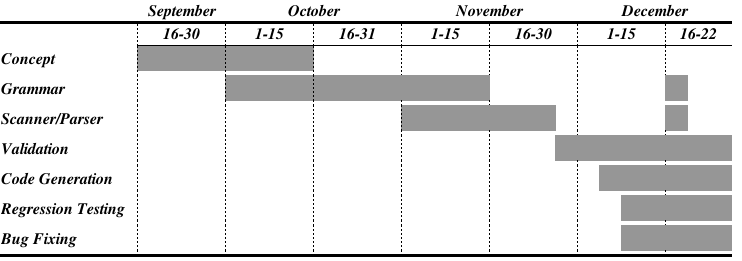
\includegraphics[scale=.5]{timeline.png}
\caption{Timeline for Setup Team}
\end{figure}

\textbf{September. } Our team held weekly meetings to discuss different potential ideas for a language.  By the end of the month, we had decided on a language that would manipulate sets.  We then set to work developing a rough draft for a working grammar and began drafting our reference manual.

\textbf{October. } In conjunction with writing the first draft of our LRM, we began work on the scanner and parser. As we built the parser, we found several areas where our grammar needed to be "improved."  The following graphic illustrates nicely how we spent October:

\tikzstyle{circ} = [circle, minimum height = 5em, minimum width = 5em, text centered, fill=blue!40, drop shadow, draw = blue]
\tikzstyle{toarrow} = [->, >= open triangle 90, thick]

\begin{center}
\begin{tikzpicture}
	\node (g) [circ] at (5,0) {Grammar};
	\node (s) [circ] at (7.5,-2.5) {Scanner};
	\node (p) [circ] at (2.5,-2.5) {Parser};
	
	\draw [toarrow] (g) -- (s) node [midway] {update};    
    \draw [toarrow] (s) -- (p) node [midway] {update};
    \draw [toarrow] (p) -- (g) node [midway] {update};
\end{tikzpicture}
\end{center}

\textbf{November. } We completed work on our parser in November and began working on validation (static semantic analysis) to perform type checking.  By the end of the month we were at the point where we could start generating code.

\textbf{December. } Writing code to generate valid C++ turned out to be more difficult than we anticipated, largely due to deep typing of nested tuples, and we continued to struggle with the Set-Builder construction mechanism.  We implemented a set class abstraction in C++ to handle some of the peculiarities of arbitrary set and tuple containers. Throughout December, we generated code and tested for bugs.


\chapter{Compiler Architecture}
The compiler consists of 5 principal components: Scanner, Parser, Validator, Code Generator and Set Class.  The Scanner receives input in the form of plain text files with \verb|.su| suffix and the compiler generates valid cpp code.  

The Code Generator uses the concrete parse tree generated from the Parser to output valid C++ code.  A polymorphic class hierarchy was implemented in C++ (Set Class component) to implement complicated Tuple and Set types.

The following lays out who worked on the various component implementations:

\begin{center}
\begin{tabular}{lc}
\toprule
\textbf{Component} &\textbf{Team Members}\\\midrule
Scanner	&Adam\\
Parser	&Adam, Ian\\
Validation &Bill\\
Code Generator &Andrew, Bill, Ian\\
Set Class &Bill, Andrew\\
Regression Suite &Ian, Bill, Andrew\\\bottomrule
\end{tabular}
\end{center}

\tikzstyle{n1} = [minimum height = 3em, minimum width = 10em, text centered, fill=blue!40, drop shadow, draw = blue, rounded corners]
\tikzstyle{n2} = [minimum height = 3em, minimum width = 10em, text centered, fill=orange!40, drop shadow, draw = orange, rounded corners]
\tikzstyle{n3} = [minimum height = 3em, minimum width = 10em, text centered, fill=black!40, drop shadow, draw = black, rounded corners]
\tikzstyle{n4} = [minimum height = 3em, minimum width = 10em, text centered, fill=green!40, drop shadow, draw = green, rounded corners]
\tikzstyle{toarrow} = [->, >= open triangle 90, thick]

\begin{figure}[h]
\label{arch}
\begin{tikzpicture}
	\node (input) [n3] at (5,2.5) {\Large infile.su};
    \node (s) [n1] at (5,0) {\Large Scanner};
    \node (p) [n1] at (5,-2.5) {\Large Parser};
    \node (v) [n2] at (0,-2.5) {\Large Validator};
	\node (cw) [n1] at (5,-5) {\Large Code Generator};
	\node (cpp) [n2] at (0,-5) {\Large Set Class };
    \node (out) [n4] at (5,-7.5) { \Large outfile.cpp };
	\node (test) [n2] at (10,-5) { \Large Regression Suite };
	
	\draw [toarrow] (input) -- (s);    
    \draw [toarrow] (s) -- (p);
    \draw [toarrow] (p) -- (v);
    \draw [toarrow] (p) -- (cw);
    \draw [toarrow] (v) -- (cw);
    \draw [toarrow] (cpp) -- (cw);
    \draw [toarrow] (cw) -- (out);
    \draw [toarrow] (test) -- (out);
    \draw [toarrow] (test) -- (cw);
\end{tikzpicture}
\caption{Overview of Setup Compiler}
\end{figure}

\chapter{Test Plan}
\chapter{Lessons Learned}

\chapter{Appendix}


\end{document}
